% !TeX spellcheck = en_US
\chapter{Related Work}\label{ch:related_work}

This chapter gives an introduction to RDF and presents the different compression algorithms discussed in the thesis.

\section{RDF}\label{sec:rdf}

RDF is a framework for structured data on the web. According to~\cite{hitzler} it can be formally described as follows. Let the following sets be infinite and mutually disjoint:

\begin{itemize}
	\item $U$ (URI references, typically represent unique entities or properties)
	\item $B$ (Blank nodes, represent an arbitrary value, necessary for displaying more complex logical statements)
	\item $L$ (Literals, represent fixed values, e.g. numbers or strings)
\end{itemize}

An RDF triple $(s,p,o) \in (U \cup B) \times U \times (U\cup B \cup L)$ displays the statement that the subject $s$ is related to the object $o$ via the predicate $p$. So a subject can be anything but a literal. A predicate can only be a URI and an object can be anything.

\subsection{Ontology}\label{sec:relatedworkOntology}
\todo{machen}

\section{HDT}\label{related_work_hdt}

HDT~(\cite{hdt}) is an approach for compressing RDF data which is directly tailored to RDF and the data compressed by it is still accessible for queries. The idea behind it is to make RDF's extensive representation more compact, thus reducing memory size. Usually, in many plain text formats for RDF (e.g. N-Triples~\footnote{https://www.w3.org/TR/n-triples/}) each triple is written down after another. This does not only require much space, but is also not good for query performance, since each single triple has to be traversed within a query execution.

It is easy to see that a more compact representation can be achieved by cleverly grouping the triples. That is exactly what HDT does. Imagine for example some triples that all have the same subject $s$. These would then be written in N-Triples as follows:

\begin{align*}
(s,p_1,o_{11}),...,(s,p_1,o_{1_{n1}}),(s,p_2,o_{2_1}),...,\\
	(s,p_2,o_{2_{n2}}),...,(s,p_k,o_{k_{n_k}})
\end{align*}
\todo{fix}

In HDT the triples are then grouped by $s$.

\begin{align*}
s \to [(p_1,(o_{1_1},...,o_{1_{n_1}})),(p_2,(o_{2_1},...,o_{2_{n_2}})),...,\\
 (p_k , (o_{k_{n_k}} ))]
\end{align*}

Since all triples have the same subject $s$, it does not have to be written down at the beginning of each triple anymore. On the second level the triples are then grouped according to the predicates. So all triples with the predicate $p_1$ come first, then all with the predicate $p_2$ and so on. Finally only the different objects have to be enumerated since the subject and predicate are already implicitly given. It will now be explained how HDT implements this mechanism.

First, all URIs and literals (which are usually quite long) are mapped to unique IDs (integers). From now on these IDs will be used. One can see the triples with the IDs in Fig.~\ref{fig:hdt_overview} on the left ('Plain Triples'). 

The above mentioned grouped representation is called 'Compact Triples' and can be seen in Fig.~\ref{fig:hdt_overview} in the middle. In the array 'Predicates' one can see the IDs of the predicates. A '0' means that from now on a new subject comes. For example, the first two entries in the 'Predicates' are linked to the first subject. At position 3 in 'Predicates', there is a '0'. Therefore, the following predicates are linked to the next subject (subject 2 in this case).

This works analogously for the objects, in the array 'Objects' the IDs of the objects are listed, and a '0' here means that from then on a new predicate comes. For instance, the first entry in 'Objects' is a '6', so the first derived triple would be $(1,2,6)$. The second entry of 'Objects' is a '0' since there is a change from predicate '2' to '3' in 'Predicates'.

The last representation of triples is called 'Bitmap Triples'.  This is a slight adaption of 'Compact Triples'. The array $S_p$ has the same content as 'Predicates', but without the zeros. That job is done by the bit-array $B_p$ in which a '1' at position $i$ means that at position $i$ in $S_p$ there comes a change of the subject (this change was previously denoted by a '0' in 'Predicates'). 

That works analogously for the objects where $S_o$ has the same content as 'Objects', but without zeros.

The advantage of 'Bitmap Triples' is that queries can be executed faster on this representation. Also, the compressed size is slightly smaller than with 'Compact Triples'. Therefore, 'Bitmap Triples' are always used in the current version of HDT.

HDT has also procedures for answering queries, but those will not be mentioned here, because the thesis will focus on HDT's compression ability.

\todo{dict compr erkären}

\begin{figure}[h]
	\centering
	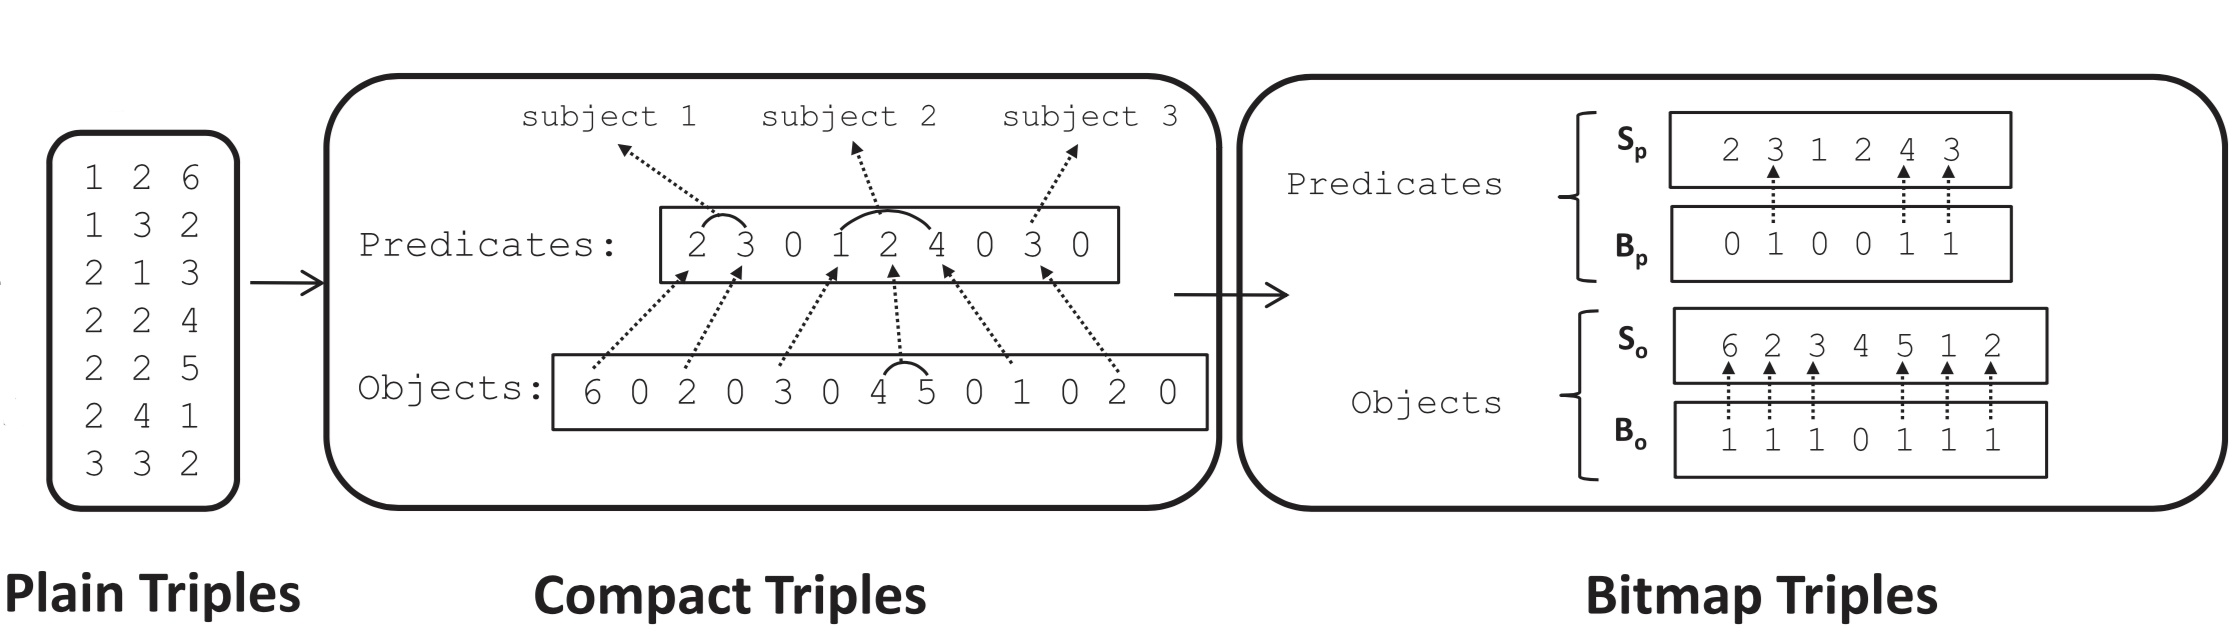
\includegraphics[width=1\textwidth]{figures/relatedwork/hdt1}
	\caption{Three different representations of triples in HDT, figure from~\cite{hdt}.}
	\label{fig:hdt_overview}
\end{figure}


\section{Grammar-based Graph Compression}\label{related_work_grammar_based}

In this section we will discuss two different approaches to grammar-based graph compression. First, ~\cite{mattdk} is introduced and briefly explained why the approach is less suitable for RDF. Then~\cite{maneth}, which the thesis will focus on, is introduced.

In general, grammar-based compressors try to find patterns that occur multiple times in the graph. Such patterns are subgraphs that can be of different kinds. Usually small patterns are searched for, since one can usually find more occurrences of these. In addition, it is possible to combine several small patterns into one large one, so that even large parts can be compressed. These small patterns are often called digrams because they consist of two elements. The exact shape of the digrams depends on the respective algorithm.

\subsection{Dürksen's Algorithm}

An approach to grammar-based compression of graphs was developed in~\cite{mattdk}. Here the authors assume a hyper graph with node and edge labels. Such a graph can be seen in Fig.~\ref{fig:transformation} on the left. To simplify the compression, a transformation is now executed, in which a new node is inserted for each edge $e$, which then has the same label as $e$. The original structure of the graph is obtained by connecting two nodes, which were previously connected by an edge, indirectly by the new node. The result of the transformation is a graph, which only has node labels, but no edge labels. Moreover, hyper edges (edges with more than two incident nodes) are no longer present due to the transformation.

\begin{figure}[h]
	\centering
	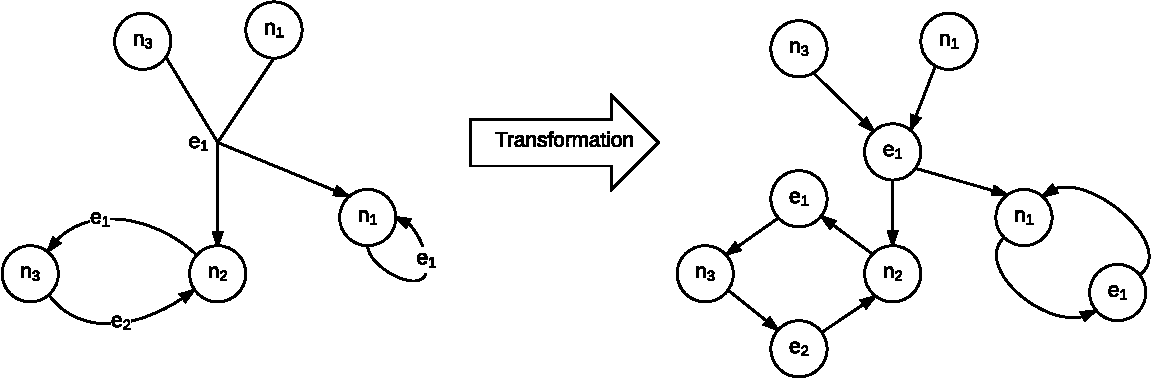
\includegraphics[width=1\textwidth]{figures/relatedwork/transf}
	\caption{Transformation of a labeled graph (each edge is replaced by a new node having the label of the replaced edge).}
	\label{fig:transformation}
\end{figure}

Thus digrams like in Fig.~\ref{fig:basicdigram} can be replaced. Here it is twice the case that a node with the label \textit{X} is connected with a node with the label \textit{Y}. This digram is then stored in a central location and can be referenced via the label \textit{X'}. Thus only two nodes remain in the compressed graph (with \textit{X'} as label) and the graph was reduced to a smaller size. There are some details which make  this digram replacement possible, but they are neglected at this point. The interested reader is referred to~\cite{mattdk}.

Dürksen's algorithm does not seem to be suitable for RDF, because it is based on the fact that there are several nodes with the same label. However, since in RDF a node represents an entity that does not occur twice, Dürksen's basic assumption is not fulfilled in RDF.

In addition, Dürksen's algorithm is not yet in a mature state, i.e., there is only a rudimentary implementation that does not work reliably for large graphs. In addition, work is currently underway to find a compact representation of such a compressed graph in order to save the data with little memory.~\cite{mattdk}

For these reasons the thesis will focus on the compressor GraphRePair, which is presented in chapter~\ref{ch:GRP}.

\begin{figure}[h]
	\centering
	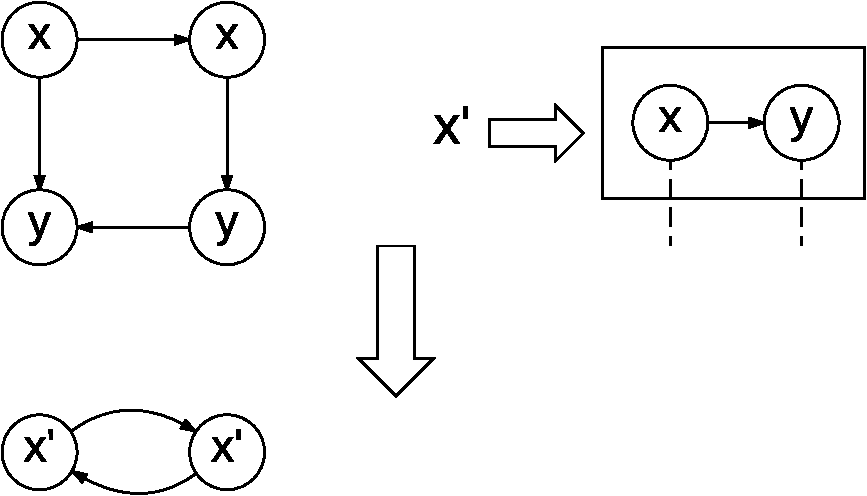
\includegraphics[width=0.6\textwidth]{figures/relatedwork/basisdigram}
	\caption{Replacement of two occurrences of the digram $X \to Y$ by nodes with the label $X'$.}
	\label{fig:basicdigram}
\end{figure}

\subsection{GraphRePair}\label{ch:GRP}

This chapter deals with GRP, the compressor from~\cite{maneth}. It firstly presents some foundations and afterwards explains what digrams and digram occurrences are in GRP. Finally, the main routine of the compressor and the encoding of the compressed data are discussed.

\subsubsection{Foundations}

For a set $M$, $M^+=\{x_1 \cdot x_2 \cdot ... \cdot x_n | x_1,x_2,..,x_n \in M \}$ is defined as the set of all non-empty strings of $M$ where $\cdot$ stands for the concatenation of two symbols.
$M^*=M^+ \cup \{ \epsilon \} $ is similar to $M^+$, but it also includes the empty string $\epsilon$.

Let $\Sigma$ be an alphabet. A hypergraph over $\Sigma$ is a tuple $g=(V,E,att,lab,ext)$ where $V=\{1,...,n\}$ is the set of nodes. $E \subseteq \{(i,j) | i,j\in V\} $ is the set of edges. $att: E \to V^+$ is the attachment mapping assigning start and end nodes to all edges. $lab: E\to \Sigma$ is the edge label mapping, and $ext \in V^*$ is a series of external nodes. A hypergraph does not contain multi-edges, which means for two edges $e_1\not=e_2$ it holds $att(e_1)\not=att(e_2) \vee lab(e_1)\not=lab(e_2)$. For a hypergraph $g=(V,E,att,lab,ext)$  $V_g, E_g, att_g, lab_g, ext_g$ are used to refer to its components.

An example for a hypergraph is illustrated in Fig.~\ref{fig:hypergraph}. Formally the graph can be described as $V=\{1,2,3\}$, $E=\{e_1,e_2,e_3\}$, $att=\{e_1 \mapsto 1 \cdot 2, e_2 \mapsto2 \cdot 3, e_3 \mapsto 2 \cdot 1 \cdot 3 \}$, $lab=\{ e_1\mapsto a, e_2 \mapsto b, e_3 \mapsto A \}$ and $ext=3 \cdot 1$.

\begin{figure}
	\centering
	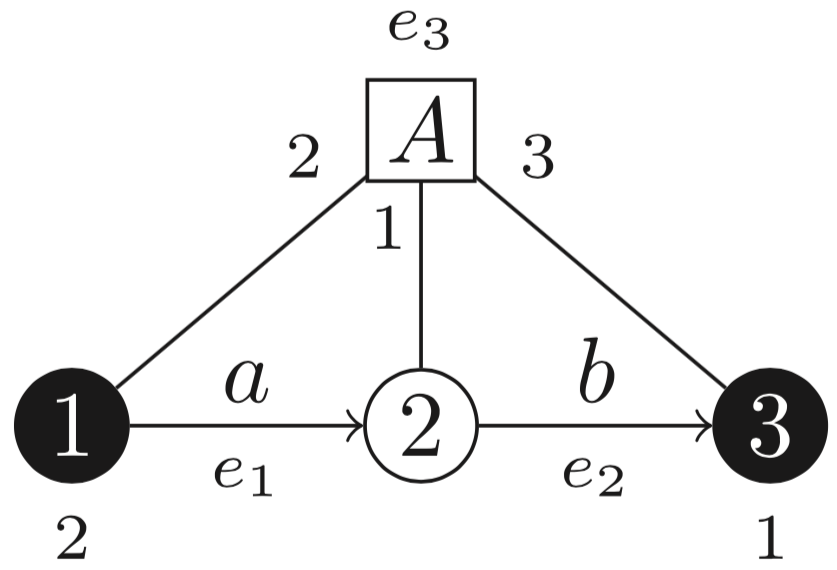
\includegraphics[width=0.3\linewidth]{figures/relatedwork/hypergraph}
	\caption{A hyper graph as defined in~\cite{maneth}. The black nodes 1 and 3 (consider the numbers within the nodes) are external nodes whereas the white node 2 is internal. $e_3$ (with the label A) is a hyper edge while $e_1$ and $e_2$ (labeled with \textit{a} and \textit{b}, respectively) are normal edges.} The numbers 2, 1 and 3 around $e_3$ denote the order of the nodes attached to $e_3$.
	\label{fig:hypergraph}
\end{figure}

External nodes are black and the numbers below them indicate indexes for their position in $ext$. Analogously,  hyper edges ($e_3$ in this case) have indexes indicating the order of the attached nodes. The utility of external nodes is explained below.~\cite{maneth}

\subsubsection{Digrams in GRP}

A digram $d$ is a hyper graph with $E_d=\{e_1,e_2\}$ so that the following conditions hold:

\begin{enumerate}
	\item $\forall v \in V_d : v\in att_d(e_1) \vee v \in att_d(e_2)$
	\item $\exists v\in V_d : v\in att_d(e_1) \wedge v\in att_d(e_2)$
	\item $ext_d \not= \epsilon$
\end{enumerate}

Condition 1 ensures that all nodes in $d$ are incident to one of the two edges of $d$. Conditions 2 is used to make sure that there is one 'middle node' incident to both edges of $d$. Finally, condition 3 ensures that there are external nodes. External nodes are not a real part of the digram, they represent other nodes of the overall graph which are connected to elements of the digram.~\cite{maneth}


\subsubsection{Digram Occurrences in GRP}

Digram occurrences are concrete instances of a digram.

Let $g$ be a hyper graph and $d$ be a digram with the two edges $e_1^d,e_2^d$. Let $o=\{e_1,e_2\} \subseteq E_g$ and let $V_o$ be the set of nodes incident with edges in $o$. Then $o$ is an occurrence of $d$ in $g$ if there exits a bijection $b:V_o \to V_d$ so that for $i\in \{1,2\} $ and $v\in V_o$ all following conditions hold:

\begin{enumerate}
	\item $b(v)\in att_d(e_i^d) \text{ iff } v\in att_g(e_i)$
	\item $lab_d(e_i^d)=lab_g(e_i)$
	\item $b(v)\in ext_d \text{ iff } v\in att_g(e) \text{ for some } e\in E_g \setminus o$
\end{enumerate}

Condition 1 and 2 ensure that the two edges of $o$ form a graph isomorphic to $d$. Condition 3 makes sure that every external node of $d$ is mapped to a node in $g$ that is incident to at least one edge in $g$ that is not contained in $o$.~\cite{maneth}

\subsubsection{Algorithm}

Algorithm~\ref{alg:GRP} is the main routine of GraphRePair. The algorithm take a graph as input and returns a grammar whereas $N$ is the set of non terminals, $P$ is the set of productions and $S \in P$ is the start production. It maintains a list of digram occurrences in $g$. As long as this list contains multiple occurrences for one digram the loop will continue. In the loop, the most frequent digram is found and then replaced and the grammar is extended. After a digram replacement the occurrence list has to be updated, because the graph has changed and former digram occurrences may not exist anymore. Moreover, new digram occurrences can be present. This occurrence update is a complex process and will not be discussed here, since it is not relevant for the thesis.~\cite{maneth}

\begin{algorithm}
	\caption{GraphRePair (Graph $g=(V,E,att,lab,ext)$)}\label{alg:GRP}
	\begin{algorithmic}[1]
		\State $ N,P\leftarrow \emptyset$
		\State $S \leftarrow g$
		\State $L(d) \leftarrow $ list of non-overlapping occurrences of every digram $d$ appearing in $g$
		\While{$|L(d)|>1$ for at least one digram $d$}
			\State $mfd \leftarrow$ most frequent digram
			\State $A \leftarrow$ new non terminal for $mfd$
			\State Replace every occurrence of $mfd$ in $g$
			\State $N \leftarrow N \cup \{A\}$
			\State $P\leftarrow P\cup \{A \to mfd \}$
			\State Update the occurrence list $L$
		\EndWhile
		\State \Return Grammar $(N,P,S)$
	\end{algorithmic}
\end{algorithm}


\subsubsection{Grammar Encoding}

After GRP has constructed a grammar for some graph, this grammar has to be stored in an efficient way. The start production (the graph) is most often much bigger than the other productions and is therefore encoded differently. 

The start production is encoded using $k^2$ trees which is illustrated in Fig.~\ref{fig:encoding}. The adjacency matrix of the compressed graph (start rule of the grammar) is considered here. First, that matrix is extended with zeros to the next power of two. Then it is partitioned into $k^2$ equally large partitions ($k=2$ here).

The tree's root represents the whole matrix and its child order correspond to the order of the just created partitions. If a partition only contains zeros, a zero leaf is added to the tree (e.g. in Fig.~\ref{fig:encoding} (a), partition 4, right bottom). Otherwise a one-node is added and the corresponding condition will be partitioned itself. The recursive procedures continues until there is zero-leaf for each path of the tree.

Afterwards, the tree is represented by bit-strings.

Since the graph has also edge labels, an adjacency matrix and its corresponding tree will be created for each of those labels.

\begin{figure}
	\centering
	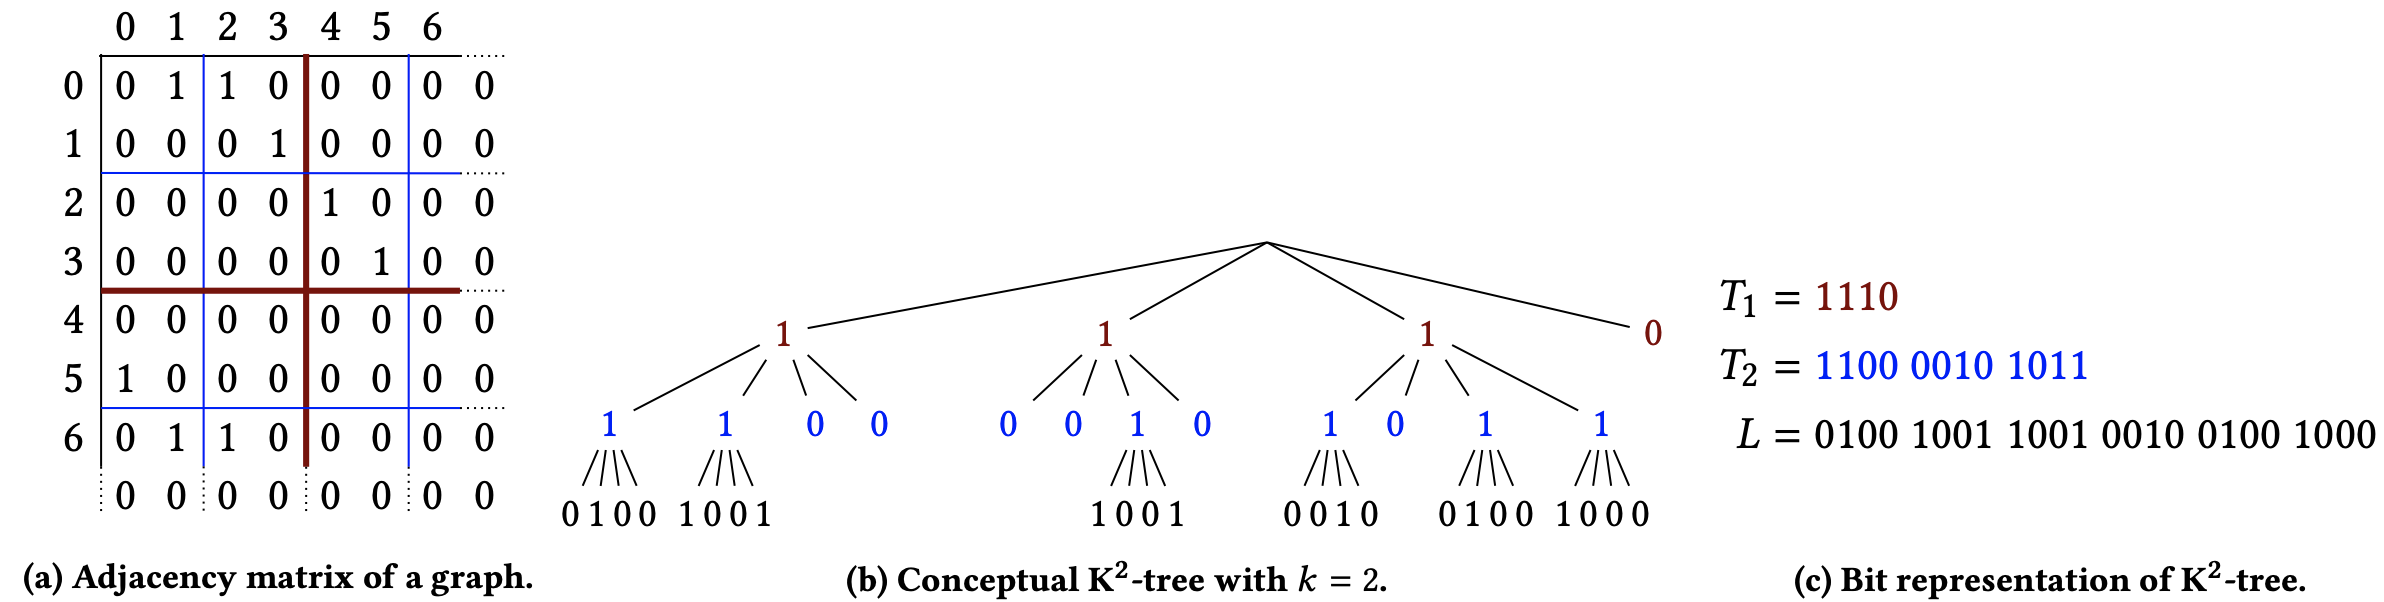
\includegraphics[width=1\linewidth]{figures/relatedwork/encoding}
	\caption{An adjacency matrix, its $k^2$ tree representation and the tree's bit representation.}
	\label{fig:encoding}
\end{figure}
\todo{einfachere Grafik oder alles erklären}

The remaining productions of the grammar are encodes differently, because they are usually quite small compared to the start production. Here, $\delta $-codes with variable length are used. Essentially this is a way of displaying numbers as a bit-string in an efficient way (similar to a Huffman Code). To realize that, the right hand side of the components of the production have to represented by numbers, e.g. the edges labels, the node IDs etc.~\cite{maneth}\todo{genauer erklären}



















